\chapter{Multi-domain semantic measures} \label{chap:multidomain}

\begin{note-paper}
    This chapter is adapted from a papers submitted to Oxford Bioinformatics in December 2015, and is still waiting its first round of peer-review reports.
\end{note-paper}

Given the multidisciplinarity of biomedical resources, it is necessary to implement measures of similarity that can handle all the relevant domains. For instance, to compare metabolic pathways one can use protein similarity~\citep{Clemente2005} or chemical similarity~\citep{Grego2010}, but we can also conceive a scenario where both sources of knowledge are important and, therefore, where comparison needs to explore the two domains. In theory, this should provide a more accurate insight into what the pathways represent in the real world and, ultimately, contribute to a better similarity measure.

In this chapter, I propose the hypothesis that multi-domain semantic similarity has some advantages compared to classical single-ontology measures when dealing with multidisciplinary resources; in particular, I demonstrate this hypothesis based on the accuracy of both techniques in the three different datasets presented in \chpref{chap:data}. By doing so, I also show that multi-domain measures are necessary for the advancement of science and that, as time passes and the amount of resources annotated with concepts from multiple ontologies increases, the demand for such measures will also increase.

Given the success of single-ontology semantic similarity measures in the past, instead of a new measure of semantic similarity built from scratch, I propose two mechanisms that \emph{lift} single-ontology measures into their multi-domain counterparts: the \emph{aggregative approach} compares each of the domains of relevance independently and then aggregates the several similarity values into a final score; and the \emph{integrative approach} integrates all the ontologies under the same common root and then applies single-ontology measures on it.

\newpage

\section{The two multi-domain approaches} \label{sec:multidomain/approaches}

Multidisciplinary entities are commonly annotated in domains that are on a one-to-one correspondence with a set of ontologies, since biomedical ontologies tend to represent a specific domain of knowledge, per the guidelines of the biomedical informatics community (see \secref{sec:concepts/ontologies} and \appref{app:ontologies}). For example, concepts used to annotate epidemiology resources include diseases from \ontology{DOID}, symptoms from \ontology{SYMP}, vaccines from \ontology{VO}, \etc. Sometimes, the same ontology corresponds to more than one domain (\eg in metabolic pathways, annotations to \ontology{CHEBI} are used both for metabolites and drugs, and \ontology{GO} annotations for molecular functions, biological processes and cellular components); the reverse is not as common (more than one ontology annotating for the same domain).

My work assumes that dividing the annotations in domains can be done in a straightforward way (\cf the datasets described in \chpref{chap:data}, where such division is presented in those chapter's tables). It also assumes the existence of a group-wise single-ontology semantic similarity measures which can compare a set of concepts with another set of concepts, examples of which include:
\begin{itemize}
    \item concept-wise similarity measures, such as $\sim[Resnik]$~(\eqref{eq:resnik-ssm}) and $\sim[Lin]$~(\eqref{eq:lin}), which can be made group-wise with the use of an aggregation technique, as described in \secref{sec:sota/annotated}; and
    \item measures that are inherently group-wise, like $\sim[UI]$~(\eqref{eq:simui}), $\sim[GIC]$~(\eqref{eq:simgic}) and $\ferreira$~(\eqref{eq:ferreira}).
\end{itemize}

The following subsections describe the two approaches that lift single-ontology measures into multi-domain measures.


\subsection{Aggregative approach} \label{sub:approaches/aggregative}

This approach treats each domain of annotation independently. For each annotation domain, the concepts of that domain used to annotate the first entity are compared to the concepts of that domain used to annotate the second entity, using the group-wise single-ontology measure. This produces a collection of similarity values, one for each domain, which must then be aggregated with the use of a function such as the maximum, the minimum or the average. See \figref{fig:aggregative} for a graphic illustration of this process.

While the aggregation technique can be one of several different options, I show here only the results of two of them: the raw average and the weighted average. Let $e$ and~$e'$ be two multi-domain annotated entities being compared, $e_d\,$ and~$e'_d\,$ be the set of concepts annotating the entities $e$ and~$e'$ in the domain~$d$, $D$~be the set of all domains annotating the two entities, and $\sigma$~be the single-ontology semantic similarity measure being lifted. I define
\begin{eqnarray}
    \sim[Aggr_{raw}](e, e') &=&
    \frac{1}{N} \cdot
    \sum_{d \in D} \sigma(e_d, e'_d)
    \label{eq:sim-aggr-raw} \\
    %
    \sim[Aggr_{weighted}](e, e') &=&
    \frac{1}{\sum_{d \in D} w_d} \cdot
    \sum_{d \in D} w_d \cdot \sigma(e_d, e'_d)
    \label{eq:sim-aggr-weighted}
\end{eqnarray}
where $w_d$~is the weight associated with the domain~$d$. I followed an approach that weights each domain by the amount of annotations that it provides to the entities being compared; as such, domains that are more represented in an entity contribute with a higher weight to the final similarity value:
\begin{equation}
    w_d = \left\vert e_d \cup e'_d \right\vert.
\end{equation}
For example, if a domain contributes to the annotations of $e$ and~$e'$ only with one concept (either only to one of the entities or to both), the weight of this domain will be~$1$. Domains that contribute with a higher number of concepts have a higher weight on the overall similarity value.

\begin{figure}
    \centering
    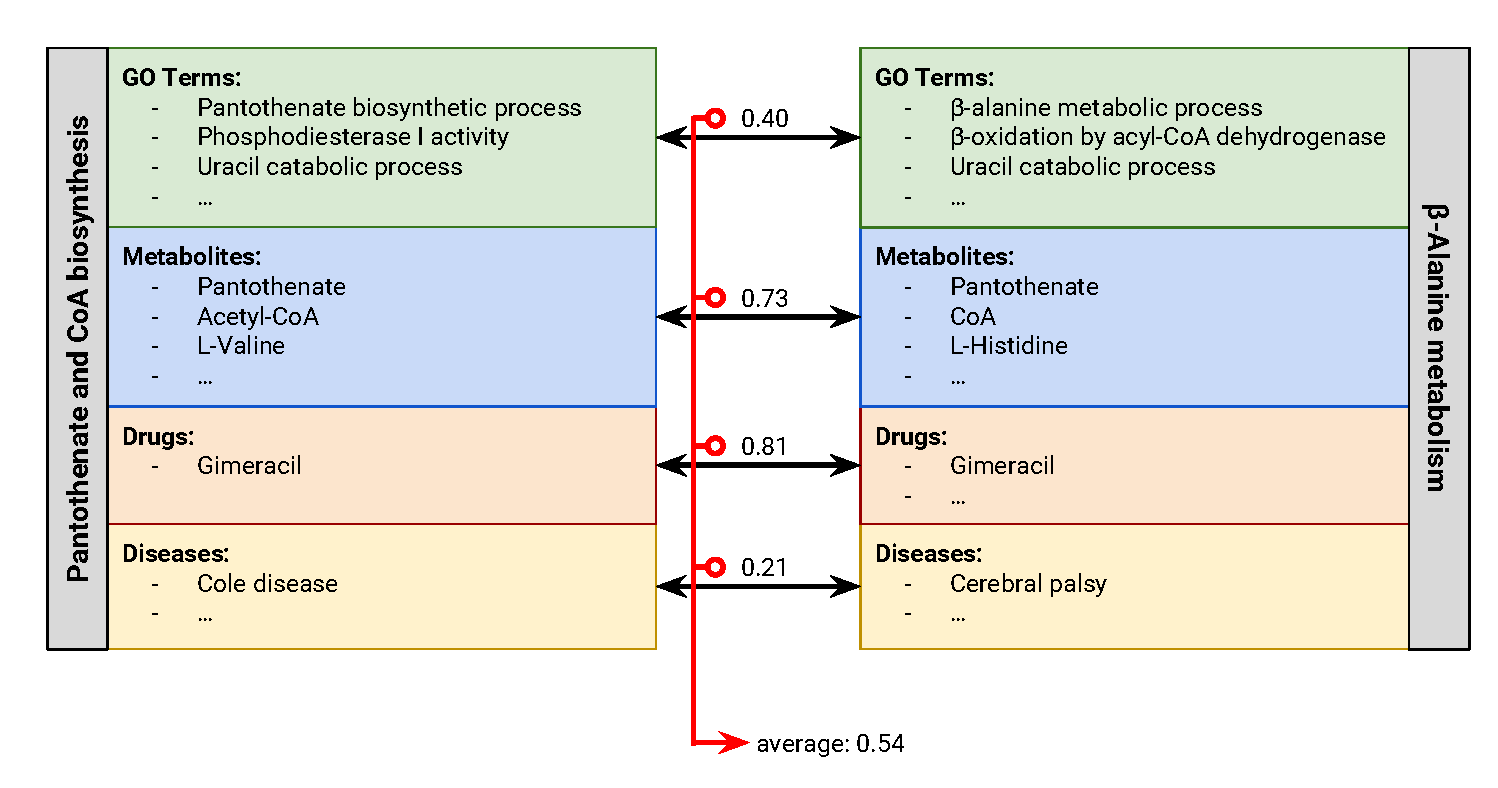
\includegraphics[width=\linewidth]{images/multi-aggregative.pdf}
    \caption[The aggregative approach]{This image illustrates how this mechanism works using two metabolic pathways as example. Each domain is identified by colour. The concepts in each domain in the first entity are compared to the concepts in the same domain in the second entity, and then the values are aggregated; in this example, the aggregation mechanism was the raw average.}
    \label{fig:aggregative}
\end{figure}

This method has the advantage that it can directly use existing measures to compute similarity and works irrespective of the degree of interoperability between the various ontologies used to annotate the entities.


\subsection{Integrative approach} \label{sub:approaches/integrative}

While one of advantage of the previous approach is the possibility to be applied to non-interoperable ontologies, biomedical ontologies are \emph{generally} interoperable in at least two ways:
\begin{itemize}
    \item the use of the Basic Formal Ontology (\ontology{BFO}) as an upper ontology~\citep{Grenon2004}, which means that concepts form different ontologies have the potential to share common superclasses (even if only general and abstract ones); and
    \item the use of cross-references between ontologies (\eg the link between a disease and the anatomical entities that it affects), which most ontologies in this field try to satisfy. This stems from the reuse of concepts from different ontologies (\eg \ontology{VO} reuses the concepts \term{Chemical entity} from \ontology{CHEBI} and \term{Protein complex} from \ontology{GO}), which enables ontologies to refer to concepts outside their domain but at the same time relevant for describing the knowledge of that domain.
\end{itemize}

In fact, by separating the various domains into independent groups, we lose information that could also be used to compute similarity. First, if only one of the entities is annotated in one domain, (\eg \ontology{FMA}), this domain is effectively ignored, and no amount of annotation can change that. Second, inter-domain relationships between concepts in different ontologies are also ignored. For example, an annotation to the concept \term{Deafness} cannot be correlated with an annotation to \term{Ear} or even \term{Hearing}, since those concepts are all part of different domains (they are, respectively, represented in, \ontology{DOID}, \ontology{FMA} and \ontology{NCIt}).

One way to avoid the pitfalls of separating the multiple domains in isolate computations is to merge all the relevant ontologies in a single multi-domain virtual ontology and then to use the single-ontology measure directly on top of this virtual ontology. This is the second approach, where all concepts of one entity are compared to all the concepts of the other (see \figref{fig:integrative}). Measures of this type assume, therefore, that there is interoperability between the ontologies being used. This is essential in two accounts:
\begin{itemize}
    \item in relatedness measures, it is vital, for example, that the molecular function \term{ATP binding} is explicitly related to the chemical compound \term{ATP}, since this relationship allows the relatedness measure to compute a high value for this pair of concepts;
    \item likewise, although the molecular functions \term{Ethanol degradation} and \term{Cellular response to ethanol}, both part of \ontology{GO}, are not fundamentally similar (one is the process by which the body converts ethanol to other smaller molecules, the other is the process that cells undergo in the presence of ethanol, and their most informative common superclass is the abstract concept \term{Physiological process}), both contribute to the metabolism of the same compound, and are similar in the sense that the two processes are related to \term{Ethanol}, a concept that is represented in a different ontology. Exploring this relationship can also increase accuracy of similarity.
\end{itemize}

\begin{figure}
    \centering
    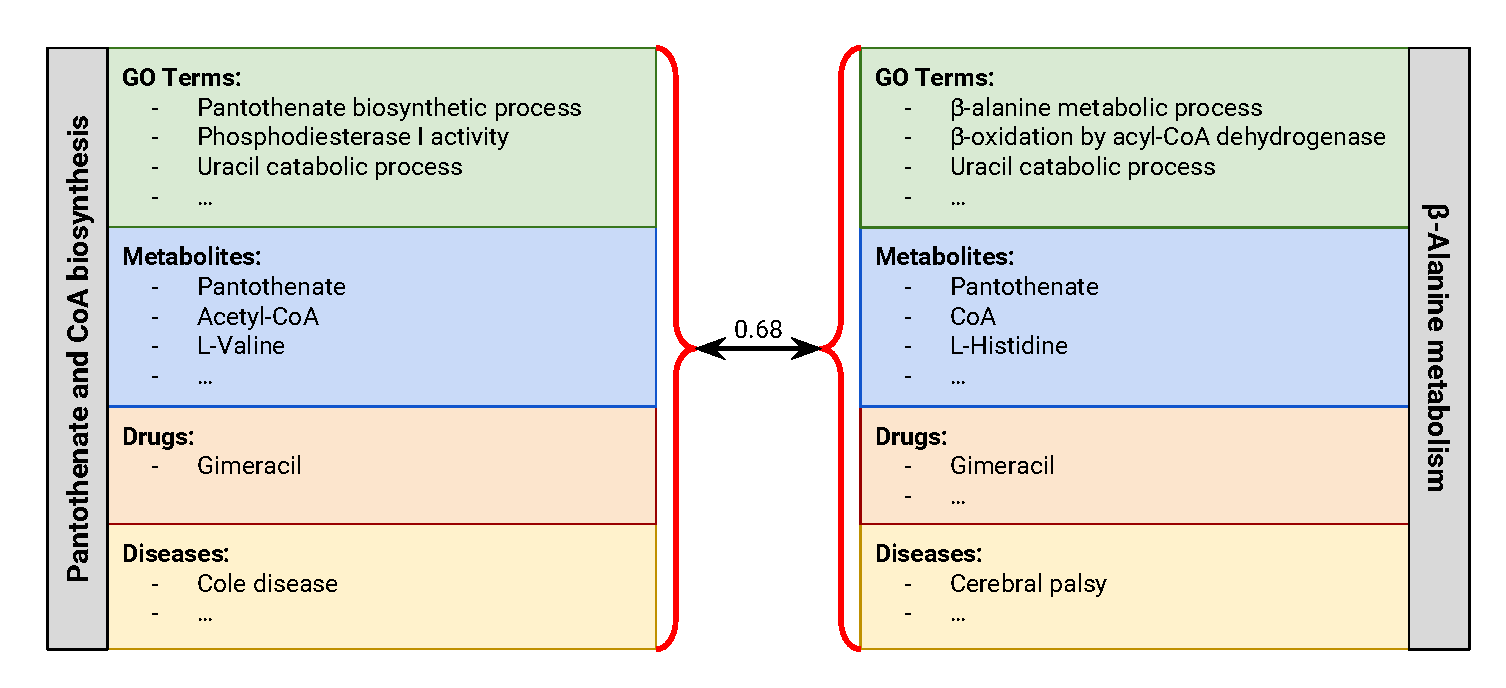
\includegraphics[width=\linewidth]{images/multi-integrative.pdf}
    \caption[The integrative approach]{All the ontologies are aggregated under the same root, which means that single-ontology measures can be directly applied to compare concepts from different domains. In this case, only one value is obtained, which corresponds to the semantic similarity value.}
    \label{fig:integrative}
\end{figure}

To achieve this, all the ontologies that are used must be in some way merged into a single knowledge representation artefact (a single ontology). Merging ontologies is a process that is mainly studied by Ontology Matching~\citep{Shvaiko2005,Euzenat2007}, and consists in automatically or semi-automatically finding the concepts that are equivalent in two ontologies. In the semantic web context (see \secref{sec:concepts/semantic-web}), ontology matching has a critical role, since it helps integrate heterogeneous entities, usually created by different research groups but with a certain overlap in their domains. However, there is a large effort to make biomedical ontologies interoperable, in the sense that
\begin{paralist}
    \item concepts are reused among ontologies to refer to the same real-world idea,
    \item there is a common upper level ontology, which represents the most abstract concepts and provides a common ontological background that enables an objective classification of concepts, and
    \item ontologies are orthogonal, thus each is responsible for representing exactly one domain of knowledge.
\end{paralist}
As such, ontology matching between reference ontologies in the biomedical domain is not expected to produce a high number of matches. In fact, since each ontology represents a different domain, there are, theoretically, no ``semantically equivalent'' concepts in any pair of reference biomedical ontologies (in practice, this is not exactly true, as some domains overlap \mdash \eg both \ontology{GO} and \ontology{FMA} contain the concept of \term{Cell}, represented with different identifiers \mdash but the amount of overlap is extremely small, it is decreasing as time goes by, and it is almost always relative to abstract rather than specific concepts).
\looseness=1

Therefore, in practice, biomedical ontologies that need concepts from other domains ``import'' those concepts from other ontologies. For example, many biological process concepts in \ontology{GO} represent biochemical reactions, and these concepts are appropriately linked to the \ontology{CHEBI} concepts that represent the molecules that are transformed in these reactions: \eg the concepts \term{Ethanol degradation} and \term{Cellular response to ethanol} mentioned above are linked to the concept \term{Ethanol} represented in \ontology{CHEBI}. These facts are asserted using existential quantification axioms (see \secref{sec:enhancements/relatedness}):
\begin{align*}
    \term{GO:``Ethanol degradation''} &
        \sqsubseteq\:\exists\,\prop{has-input}\,.\,\term{CHEBI:``Ethanol''}, \\
    \term{GO:``Cellular response to ethanol''} &
        \sqsubseteq\:\exists\,\prop{has-input}\,.\,\term{CHEBI:``Ethanol''}.
\end{align*}

Rather than ontology matching, it is these inter-domain cross-references that can potentially increase the accuracy of semantic similarity measures. With them, it becomes possible to find a specific rather than abstract connection between the \ontology{GO} concepts \term{Ethanol degradation} and \term{Cellular response to ethanol}, which was otherwise absent from the \ontology{GO} ontology. Measures such as~$\ferreira$ are capable of exploring the inter-domain cross-references and use them to compare ontology concepts (see \secref{sec:enhancements/relatedness}) and, by extension, annotated entities.

% For example, a mapping from diseases to frequently associated symptoms is useful when comparing entities associated with diseases \andor symptoms. One the one hand, this provides a means to directly measure relatedness between a disease and a symptom; on the other hand, similarity between diseases can also reflect the real world more accurately, since more information is added to the system and can be used for that comparison (\eg measures that are able to exploit this kind of information can assign a higher value to the similarity between diseases that share frequent symptoms, even if the diseases are otherwise not similar).

Unfortunately, the current state of cross-linking in biomedical ontologies is largely underdeveloped, despite it being a recommended practice by the OBO Foundry. The group responsible for developing and maintaining \ontology{GO} intends to provide cross-references to appropriate concepts from other ontologies. Examples already deployed are the ones given in the previous paragraph, which link \ontology{GO} and \ontology{CHEBI}. Planned links include cross-references to anatomical locations and species names~\citep{Mungall2011}. Furthermore, \ontology{HPO} represents human phenotype abnormalities, and links them to anatomical concept from \ontology{FMA}. For example, \term{Microtia} is defined as the ``Underdevelopment of the `external ear' (\ontology{FMA}:52781)''.

Incidentally, OWL is well suited to deal with this type of cross-reference. If two ontologies refer to the same identifier, when the ontologies are used together, that identifier will refer to the same concept; as long as all the necessary ontologies are loaded, these type of inter-domain axioms can be defined in one ontology using an identifier from another ontology, which makes this multidisciplinary fact directly available out of the box. This is because, in the semantic web, identifiers are universal, and always identify the same concept. For example, there is an OWL file representing \ontology{GO} that contains the axioms exemplified above, which relate molecular functions with chemical compounds. This file does not have any information about the \ontology{CHEBI} concepts other than the identifier. Therefore, an automatic system that needs more information on those \ontology{CHEBI} concepts, \eg its superclasses, name and synonyms, must load \ontology{CHEBI} to find it.


\section{Results} \label{sec:multidomain/results}

I have applied semantic similarity to the multi-domain datasets described in \chpref{chap:data}. As these are intrinsically multidisciplinary datasets, they provide an appropriate and highly relevant testbed to try the two approaches described above. I refer the reader to \tabref{tab:epiwork-summary} (page~\pageref{tab:epiwork-summary}), \tabref{tab:pathways-summary} (page~\pageref{tab:pathways-summary}) and \tabref{tab:biomodels-summary} (page~\pageref{tab:biomodels-summary}), describing the amount of annotations on these datasets, which will, therefore, be pertinent to the analysis presented here.

Except where otherwise stated, all the results presented in this section were obtained using $\sim[Resnik]$~(\eqref{eq:resnik-ssm}) as the group-wise single-ontology semantic similarity measure. Since this is a concept-wise measure, I used it to create a similarity matrix, where each value is the similarity between one of the annotations in the first entity and one of the annotations in the second entity, and then use a Best Match Average (BMA) approach to convert this matrix into a single similarity value. Other group-wise single-ontology measures have been used, in particular~$\ferreira$, with results equivalent to the ones presented. As such, these results are not shown, except where relevant. In particular, although some measures are better suited to tackle some problems than other measures (for example, a measure that uses disjointness axioms is better suited to deal with problems related to \ontology{CHEBI} concepts, as detailed in \secref{sec:enhancements/disjointness}), the increase in performance observed in multi-domain semantic similarity over single-ontology semantic similarity is largely independent of the group-wise measure used with it.

For each case study, I used semantic similarity in four different settings:
\begin{description}
    \item[Baseline] This is a collection of measures instead of a single one. Each measure compares only the concepts from one domain and completely disregards the other domains. This corresponds to the classical single-ontology measure and serves as a baseline to determine whether multi-domain measures outperform single-ontology measures.
    \item[Aggregative (raw)] This setting corresponds to the aggregative approach, with all the single-ontology values obtained in the baseline setting being averaged with equal weights~(\eqref{eq:sim-aggr-raw}).
    \item[Aggregative (weighted)] This is the same as last setting, except that the average of the various values is weighted in proportion to the number of annotations in each domain~(\eqref{eq:sim-aggr-weighted}).
    \item[Integrative] This corresponds to the integrative approach. All the ontologies relevant for the similarity calculation are merged into one ontology and then the single-ontology measure is applied to it.
\end{description}


\subsection{Epidemiology Dataset} \label{sub:results/epiwork}

Among the annotations for the $228$~epidemiology-related papers uploaded to the Epidemic Marketplace, there are annotations made to concepts from the \ontology{NCIt} and \ontology{MeSH}. These two ontologies are much less formal than the rest of the ontologies in this dataset (see \secref{sec:concepts/ontologies} and \figref{fig:spectrum}). They are also quite broad in their scope. In fact, \ontology{MeSH} was first introduced as a means to annotate biomedical articles~\citep{Rogers1963} and \ontology{NCIt} for annotating cancer-related results~\citep{Coronado2004}; both endeavours need, therefore, a wide range of relevant biomedical concepts. For example, \ontology{NCIt} covers clinical care, translational and basic research, public information and administrative activities. As such, we can expect that the two vocabularies in fact contribute a bit to all the domains of the epidemiology resources, rather than being specific to one domain. Although these two vocabularies were originally intended to be used in the Epidemic Marketplace only when the other ontologies did not have the necessary concepts, especially as a source of non-biomedical-specific concepts (\eg ``Family characteristics'', which belongs to the socio-economic sub-domain of epidemiology), they ended up providing the majority of annotations in the dataset (\cf the columns ``Volume'' and ``Diversity'' in \tabref{tab:epiwork-summary}).

For these reasons, I calculated semantic similarity and analysed the results in two different ways: first considering all the annotations and second by ignoring the \ontology{MeSH} and \ontology{NCIt} annotations. A third study could have been performed, where the \ontology{MeSH} and \ontology{NCIt} annotations were redistributed among the actual domains they belong too, but this study was not possible, as there is no obvious means to automatically detect which domain each of these concepts belongs to.

While \tabref{tab:epiwork-summary} contains the statistics for all ontologies, \tabref{tab:epiwork-purge} contains the statistics for the purged dataset, where \ontology{MeSH} and \ontology{NCIt} annotations were removed, as well as the resources that were only annotated with these ontologies.

\begin{table}
\caption[Summary of the annotation in the purged epidemiology dataset]{Among the $228$~resources in the regular dataset, $68$~have annotations only to concepts in \ontology{MeSH} and \ontology{NCIt} and were, therefore, removed from this dataset, resulting in a total of $160$~resources. \Cf \tabref{tab:epiwork-summary}.}
\label{tab:epiwork-purge}
\centering
\small
\begin{tabular}{llrrr}
\toprule
\textbf{Domain} & \textbf{Ontology} & \textbf{Coverage} & \textbf{Volume} & \textbf{Diversity} \\
\midrule
Chemistry    & \ontology{CHEBI} &  1.2\% & 1.00 &  1 \\
Diseases     & \ontology{DOID}  & 57.6\% & 1.58 & 45 \\
Environment  & \ontology{ENVO}  & 30.0\% & 1.00 &  9 \\
Phenotypes   & \ontology{PATO}  &  1.2\% & 1.00 &  1 \\
Symptoms     & \ontology{SYMP}  & 65.6\% & 3.55 & 79 \\
Transmission & \ontology{TRANS} & 60.6\% & 1.00 &  9 \\
Vaccines     & \ontology{VO}    & 29.4\% & 1.06 & 16 \\
\bottomrule
\end{tabular}
\end{table}

Validation of semantic similarity in this dataset was done by determining the degree to which it is possible to predict the diseases (the \ontology{DOID} annotations) from the rest of the annotations. The reason to chose this method was that performing a clinical diagnosis is equivalent to predicting the diseases based on the other known factors (most notably symptoms) and is, therefore, one of the most important problems in biomedical informatics. According to the hierarchy developed in \chpref{chap:validation} and illustrated in \figref{fig:hierarchy}, this validation strategy is classified into the ``Classification prediction for single entities'' branch.

To this purpose, I used a multi-label machine learning algorithm named~ML-KNN, described by \citet{Zhang2007} and based on the more general algorithm known as $k$-nearest neighbours~(\knn). ML-KNN operates approximately as follows:
\begin{enumerate}
    \item For each resource~$r$, compare it to all other resources using semantic similarity without using the \ontology{DOID} annotations, and find the $k$~resources most similar to~$r$.
    \item Build a Bayesian network classifier~\citep{Friedman1997} based on the frequency with which each \ontology{DOID} concept appears in the $k$~neighbours.
    \item Use the classifier to calculate the probability that each \ontology{DOID} concept is one of the annotations of~$r$; let $p_r(d_i)$~be the probability associated with concept~$d_i$ in resource~$r$.
    \item For each resource, sort the \ontology{DOID} concepts according to their associated probability.
\end{enumerate}

Evaluation of this approach can be measured with a number of different methods, making use of the following notation:
\begin{itemize}
    \item $R$ is the set of all resources in the dataset;
    \item $D$ is the set of all \ontology{DOID} concepts;
    \item $C_r \subseteq D$ is the set of \ontology{DOID} concepts annotating~$r$, \ie the set of correct labels; and
    \item $I_r = D \setminus C_r$ is the set of concepts not used to annotate~$r$, \ie the incorrect labels.
\end{itemize}
I assessed the performance of each semantic similarity measure using an evaluation measure adapted from~\citet{Zhang2007} (therein named ``coverage''), described as:
\begin{equation}
    E = \frac{1}{\left\vert R\right\vert} \cdot
    \sum_{r\in R} \frac
        {\left\vert\left\{d_i\in I_r\mid p_r(d_i) < m_r\right\}\right\vert}
        {\left\vert I_r\right\vert}
\end{equation}
where $m_r=\min\left\{p_r(d_i)\mid d_i\in C_r\right\}$. This calculates, for each resource~$r$, the fraction of incorrect labels of~$r$ that have a low probability associated with it, setting the threshold to the value of the lowest probability of any correct label. In this sense, it is analogous to the specificity at the level of perfect recall: we expect that the number of incorrect labels after the threshold~$m_r$ is as high as possible. The perfect similarity measure would completely separate the expected \ontology{DOID} labels from the incorrect ones, resulting in an evaluation~$E=1$.

Other evaluation measures can be applied to this problem. For example, the original ML-KNN paper proposed to measure the fraction of resources for which the most probable label is indeed an expected label, or the fraction of pairs of expected \vs incorrect labels where the probability of the correct label is higher than the probability of the incorrect label. All these evaluation measures point to the same conclusions that I present here and, as such, are not shown.

\begin{figure}
    \centering
    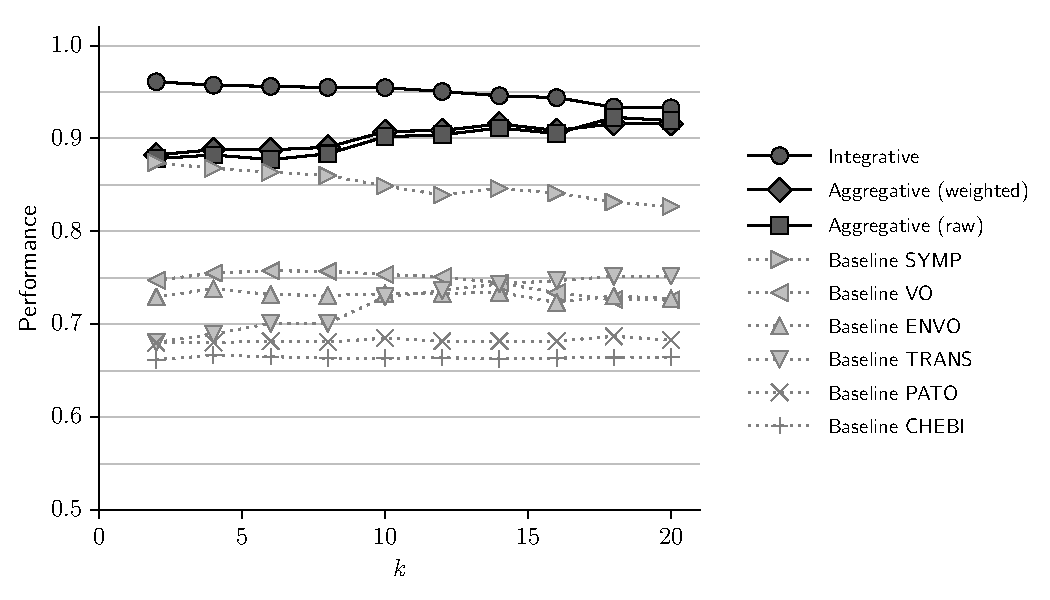
\includegraphics[width=0.9\linewidth]{images/epidemic-purge-resnik.pdf}
    \caption[Semantic similarity in the purged Epidemic Marketplace dataset]{These results show the performance of the semantic similarity measures using the various settings detailed in the beginning of this section. This graph was obtained using the purged dataset, \ie excluding \ontology{MeSH} and \ontology{NCIt} annotations. Baseline settings are presented as dotted grey lines, and the multi-domain settings as black solid lines.}
    \label{fig:epiwork-purge}
\end{figure}

\begin{figure}
    \centering
     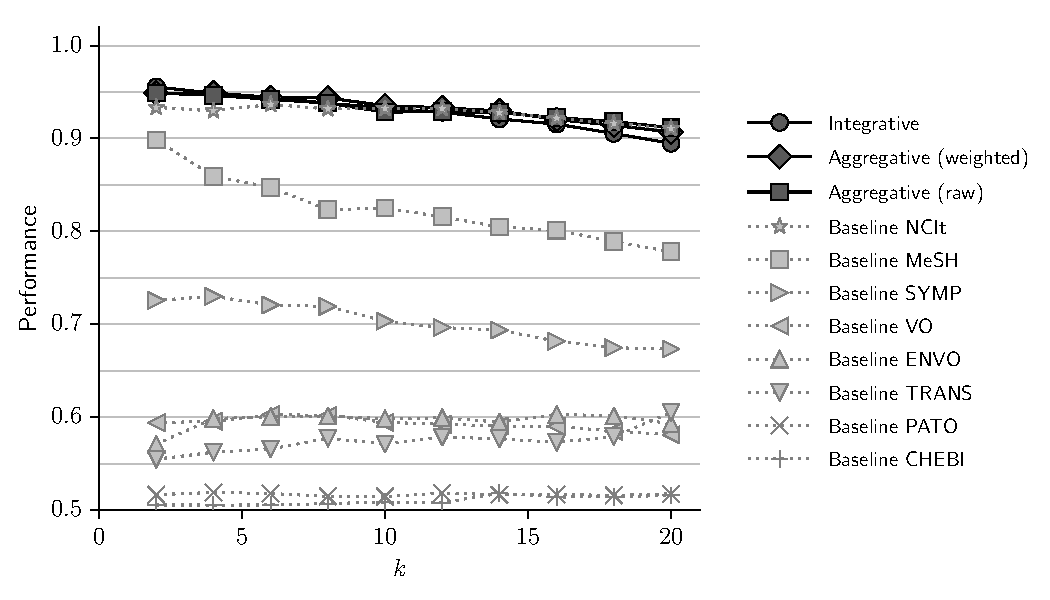
\includegraphics[width=0.9\linewidth]{images/epidemic-regular-resnik.pdf}
    \caption[Semantic similarity in the raw Epidemic Marketplace dataset]{These results show the performance using the various settings detailed in the beginning of this section. This graph was obtained using all annotations, including \ontology{MeSH} and \ontology{NCIt}. Baseline settings are presented as dotted grey lines, and the multi-domain settings as black solid lines.}
    \label{fig:epiwork}
\end{figure}

The graph presented in \figref{fig:epiwork-purge} depicts this evaluation measure with respect to the several similarity settings defined in this section, using various values of~$k$ in the ML-KNN algorithm. As can be seen, the integrative approach always outperforms the other settings, independently of the value of~$k$, thus showing the superiority of multi-domain semantic similarity in this dataset over single-ontology measures. We can observe that the single-ontology measure performed on the \ontology{SYMP} baseline (using the symptoms ontology) is the most successful baseline. This is justified by considering the annotation profile shown in \tabref{tab:epiwork-purge}. In fact, except for \ontology{DOID}, this is the domain with the highest coverage and the highest volume of annotation.

Additionally, from the set of domains used to annotate these resources, symptoms are the most closely related to diseases. This baseline shows a performance comparable to the \textbf{Aggregative} approaches, especially for low values of~$k$, which means that the other domains have little to add to the information already provided by \ontology{SYMP} (the gap increases with the increase of~$k$). However, the \textbf{Integrative} approach shows a higher performance than the other multi-domain approaches for all values of~$k$. This may be justified with the fact that many resources are annotated with different sets of domains. For example, consider the calculation of similarity between a resource that has annotations from \ontology{TRANS} with a resource with \ontology{TRANS}, \ontology{SYMP} and \ontology{VO} annotations. In the \textbf{Aggregative} approaches, only the \ontology{TRANS} domain can be used, which results in the method ignoring some annotations; but the \textbf{Integrative} approach uses all annotations, irrespective of domain, thus being able to more correctly discern between the resources and being, in general, more accurate. This appears to be an especially relevant result in this dataset, as the coverage of the various domains is small.
\looseness=1

% On the one hand, we need to consider the ``noise'' introduced into the multi-domain measure by the other ontologies. For example, similarity measured in the \ontology{TRANS} domain performs poorly, even though it is used to annotate a significant fraction of the resources ($60.6\%$). However, only $9$~distinct concepts are used for this domain, which means that its discriminating power is severely affected when compared, for instance, to the \ontology{VO} domain (lower coverage but higher diversity). Thus, introducing these annotations into the multi-domain measure does not increase the performance significantly.

\figref{fig:epiwork} contains an equivalent graph, obtained in the regular dataset (including \ontology{MeSH} and \ontology{NCIt} annotations). Notice that the baseline performances are not the same as in the previous purged dataset, because this raw dataset contains more resources, specifically more resources that do not have annotations in the domains of those baselines, decreasing their performance. The main conclusion that can be taken from this result is that similarity calculated with multi-domain approaches performs as well as the best baseline (calculated with the \ontology{NCIt} domain). On the one hand, this domain corresponds to the maximum coverage, volume and diversity (see \tabref{tab:epiwork-summary}), and as such the rest of the domains have little information to add to it. On the other hand, these other domains manage to avoid adding noise to the multi-domain measures: multi-domain measures never show a performance significantly lower than the \ontology{NCIt} baseline. As expected, the best baselines correspond to the two ontologies that span all the domains of annotation.
\looseness=1


\subsection{Metabolic Pathways Dataset} \label{sub:results/pathways}

KEGG pathways are manually classified into $33$~distinct groups. For example, ``Lysine degradation'' is classified into the ``Amino acid metabolism'' group, since Lysine is an amino acid. I exploited this classification in evaluating the performance of semantic similarity in the metabolic pathways dataset by using the similarity values to predict that same manual classification. As above, this is a strategy that belongs to the ``Classification prediction for single entities'' branch of the validation hierarchy. Specifically, I applied the machine-learning algorithm $k$-nearest neighbours (\knn) to predict the class of each pathway given its similarity with the other pathways. The algorithm can be approximately described as follows:
\begin{enumerate}
    \item For each pathway~$p$, compare it to all other pathways using semantic similarity, and find the $k$~pathways most similar to it. Call this group of neighbour pathways $Q_p = \{q_1, \dots, q_k\}$.
    \item Find the class of each of these neighbours, $C(q_i)$ for~$i=1,\ldots, k$.
    \item For each class~$c'$ among all the $33$~above, count the number of neighbour pathways in~$Q_p$ that are part of that class: $f(c') = |\{q_i \in Q_p \mid C(q_i) = c'\}|$.
    \item Select~$c = \argmax_{c'}f(c')$, \ie the most common class among the $k$~neighbours. In case of a tie, the selected class is the one with a higher sum of the similarities between $p$ and the pathways in that class.
    \item Each pathway is then classified as ``correct'' if the selected class corresponds to the real one, and ``incorrect'' otherwise.
    \item Performance is reported as the fraction of correct pathways.
\end{enumerate}

As can be seen from \figref{fig:pathways}, performance was calculated for various values of~$k$, and in almost all cases we observe that multi-domain settings outperform single-ontology ones.

A conclusion that can be taken from this figure is that the different domains perform differently from one another, with the ``\ontology{GO} terms'' baseline performing on par with the \textbf{Aggregative(raw)} multi-domain setting. I refer the reader again to \tabref{tab:pathways-summary} (page~\pageref{tab:biomodels-summary}), which summarises the annotations in each domain. For example, only~$42.4\%$ of the pathways contain information on drugs, which means that only about~$18\%$ of all the pairs of pathways can use this information. Thus, using this domain results in low performance, as expected. On the other hand, all pathways are annotated with \ontology{GO} concepts, with a volume of about $30$~concepts per pathway. This, coupled with the fact that semantic similarity in the biomedical domain has been initially explored in \ontology{GO} and has been since thoroughly studied in this ontology more than in the other ontologies, means that it is not surprising that there is little improvement when going from the \ontology{GO} baseline to the multi-domain approaches. Nonetheless, improvements are observed in multi-domain settings for most values of~$k$.

\begin{figure}
    \centering
    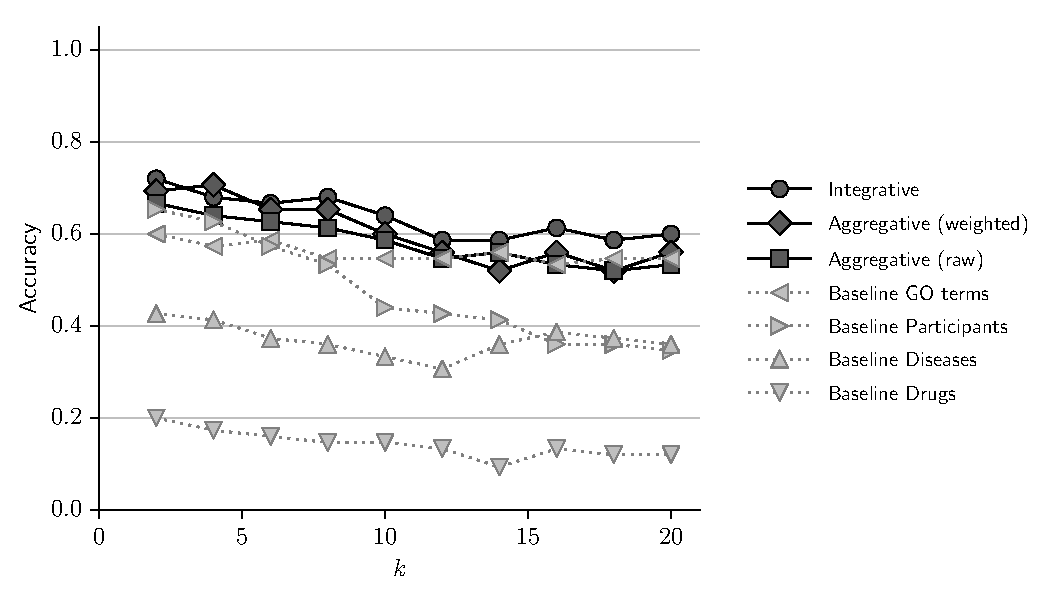
\includegraphics[width=0.9\linewidth]{images/pathways-resnik.pdf}
    \caption[Semantic similarity in the Metabolic Pathways dataset]{These results show the fraction of pathways correctly classified, using the various settings detailed in the beginning of this section. Baseline settings are presented as dotted grey lines, and the multi-domain settings as black solid lines.}
    \label{fig:pathways}
\end{figure}

\begin{figure}
    \centering
    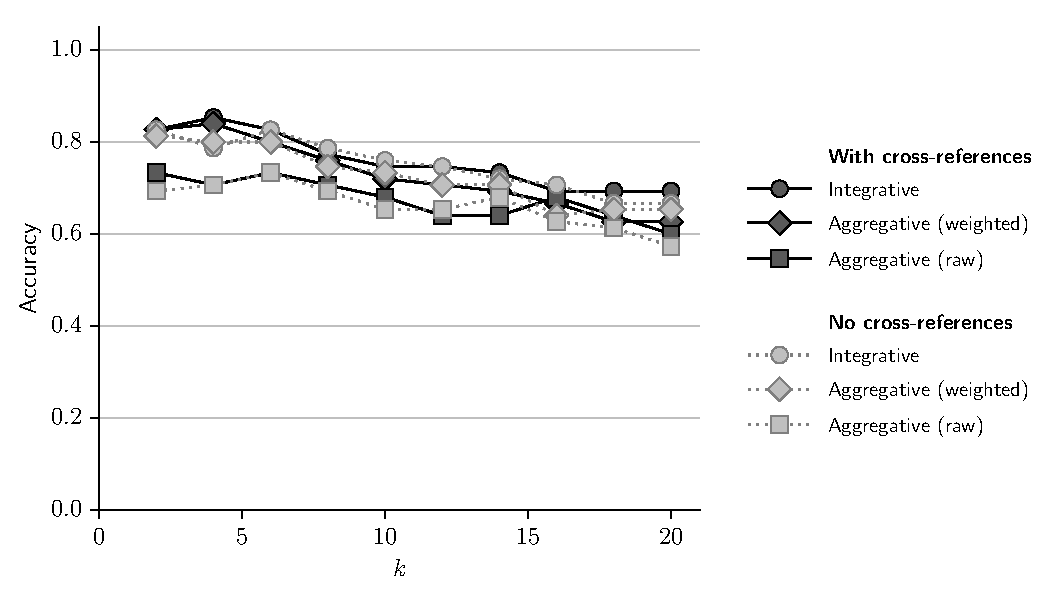
\includegraphics[width=0.9\linewidth]{images/pathways-ferreira-xref-noxref.pdf}
    \caption[Effect of cross-references on the performance of semantic similarity]{As before, these results show the fraction of pathways correctly classified, but now using only the multi-domain approaches. The black solid lines show the results obtained using the cross-references that connect the \ontology{GO} and \ontology{CHEBI} ontologies; the dotted grey lines represent the results obtained without those cross-references. Only the $\ferreira$ measure can make actual use of the cross-references, and as such this graph shows the results obtained with that measure.}
    \label{fig:xref-pathways}
\end{figure}

Unlike what happens in the previous dataset, the \textbf{Integrative} setting does not clearly outperform the other multi-domain measures. I justify this observation with the fact that the domains in this dataset are more well-balanced than in the previous one, since a majority of the pathways are annotated in a significant portion of the domains ($70\%$~of the pathways have annotations in $3$ or~$4$ domains). The ``Participants'' baseline also shows a high accuracy: it was already established that semantic similarity is a useful technique in \ontology{CHEBI}~\citep{Ferreira2010,Ferreira2013}. While the accuracy for the ``Metabolites'' and the ``Drug'' baselines is low, coupling this information with the other domains increases the performance with respect to the best baseline, namely in the \textbf{Aggregative(weighted)} and \textbf{Integrative} approaches.

In cases like these, where the domains are balanced in terms of number of annotations, and are known to produce good results with semantic similarity, I anticipate that there is no way, short of actually evaluating the results of semantic similarity, to determine which of the multi-domain approaches will lead to the best performance. Even so, I expect that at least the integrative approach will always outperform the best single-ontology baseline.

\begin{figure}
    \centering
    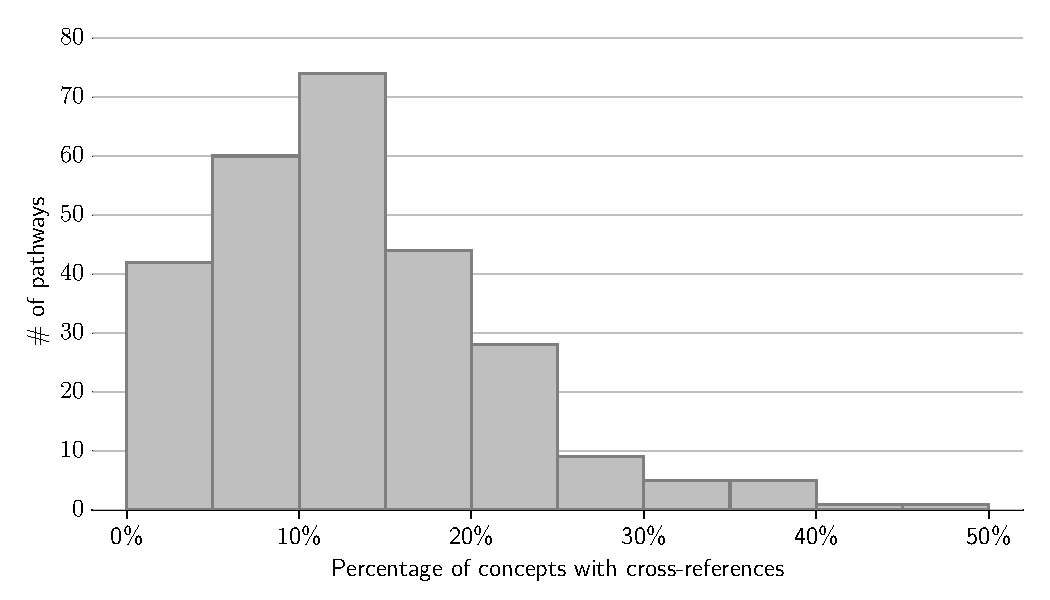
\includegraphics[width=0.9\linewidth]{images/pathways-xref-histogram.pdf}
    \caption[The distribution of the percentage of annotations that have cross-references]{This histogram plots the amount of pathways, among the $269$ in the Metabolic Pathways dataset, according to how many of their annotations have inter-ontology cross-references.}
    \label{fig:xref-histogram}
\end{figure}

As hinted before, it is also relevant to study the effect that multi-domain cross-references have on semantic similarity. Since $\sim[Resnik]$ is agnostic to cross-references, I used instead my own measure of relatedness,~$\ferreira$ (\secref{sec:enhancements/relatedness}). Given that using the links between ontologies means that the semantic relatedness algorithm has more information to work with, I originally expected that measures using cross-references would have a higher performance. \figref{fig:xref-pathways} shows the reverse: adding cross-references to the store of information accessible to the algorithm has no significant impact on the performance. The main reason for this result seems to be that the amount of cross-references is still low, when compared to the size of the dataset and the size of the ontologies. For example, cross-references exist only in \ontology{GO} ontology, and only for $25\%$~of its concepts (corresponding to only approximately~$11\%$ of the concepts of all domains). \figref{fig:xref-histogram} shows that in the majority of pathways, only~$15\%$ of the annotations have disjointness information.

On the other hand, this relatedness algorithm has been validated in \ontology{FMA} measures, which may also contribute to it not being able to use the information from \ontology{GO} cross-references. In fact, while $\ferreira$ outperforms $\sim[Resnik]$ by a large amount (\cf the results in \figref{fig:pathways} and \figref{fig:xref-pathways}, where we can see that the \textbf{Integrative} approach has accuracy values ranging in the interval~$(0.6, 0.7)$ for $\sim[Resnik]$ and in the interval~$(0.7, 0.8)$ for $\ferreira$), it seems to be unable to use the cross-references to improve its results even further.


\subsection{Biochemical Models Dataset} \label{sub:results/biomodels}

To evaluate semantic similarity in this dataset, I asked a Systems Biologist (Dr Bernard de Bono from University London College) to evaluate a predetermined set of $250$~pairs of biomodels, each according to how similar the two biomodels in the pair are (see \secref{sec:data/biomodels} and \figref{fig:biomd}).

To assess the performance of each semantic similarity measure, I evaluated the degree to which the measures reflect the manual similarity values, an approach that is classified, according to the hierarchy in \figref{fig:hierarchy}, as a ``Correlation with a manual anchor measure''. Since the gold-standard values are not continuous but rather ordinal, this correlation cannot be measured with Pearson's correlation coefficient, but should instead be measured with non-parametric coefficients such as Spearman's rank coefficient or Kendall's~$\tau$ coefficient. The results shown in this section correspond to Spearman's rank coefficient, but the ones obtained with Kendall's coefficient are equivalent in all aspects.

As can be seen from \figref{fig:biomodels}, the integrative approach outperforms all the other settings, namely the single-ontology ones. In this case, it is even more interesting to compare the results obtained with $\sim[Resnik]$ \vs $\ferreira$ (see \figref{fig:biomodels-ferreira}). The most noticeable difference is that the \textbf{Integrative} approach achieves a much higher performance with $\ferreira$ than with $\sim[Resnik]$, even though the single-ontology baselines and the aggregative approaches do not exhibit as large an increase. This seems to indicate that this multi-domain approach is able to thoroughly explore the multidisciplinarity with this measure in a way that it cannot with $\sim[Resnik]$.

\begin{figure}
    \centering
    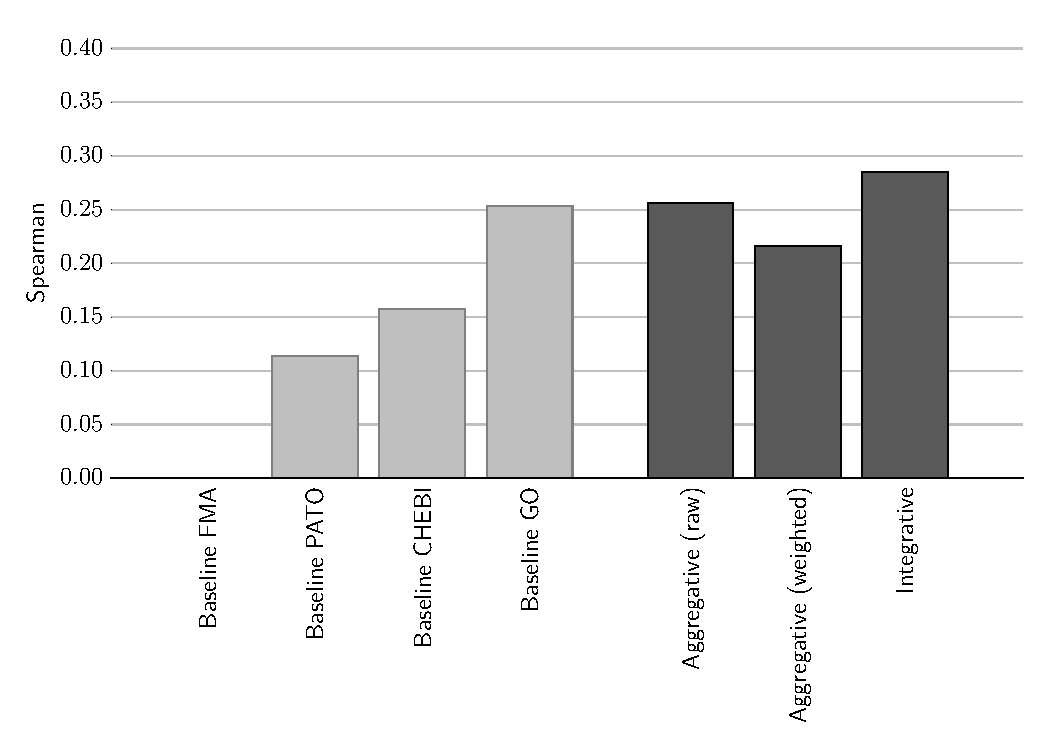
\includegraphics[width=0.9\linewidth]{images/biomodels-resnik.pdf}
    \caption[Semantic similarity in the Biochemical Models dataset with~{\boldmath$\protect\sim[Resnik]$}]{These results show the Spearman's rank coefficient between each semantic similarity measure and the gold-standard, measured with $\sim[Resnik]$. In general, the multi-domain measures (shaded in a darker tone of grey) outperform the single-ontology ones (shaded in a lighter tone of grey).}
    \label{fig:biomodels}
\end{figure}

Like in the previous dataset, \ontology{GO}-based semantic similarity performs highly (even higher than the \textbf{Aggregative} approaches). I argue that this happens for the same reasons: semantic similarity has been studied to a higher degree of detail in \ontology{GO} than in the other ontologies, and the coverage and volume of \ontology{GO} annotations is higher than the rest of the domains. In particular, semantic similarity in \ontology{FMA} yields a performance of $0$~because, even though $11$~models contain \ontology{FMA} annotations (see \tabref{tab:biomodels-summary}, the gold standard never pairs one of these $11$~models with another one of them.

Like in the first dataset, there is a discrepancy between the three multi-domain settings, as the integrative approach outperforms the \textbf{Aggregative} ones. I believe the reasons for this are equivalent to the ones presented before: in the \textbf{Aggregative} approach, the final similarity score will be an average of four measures, three of which exhibit a low performance. It is not surprising, therefore, that its performance does not increase much with respect to the ``\ontology{GO}'' baseline (in fact, performance decreases for the \textbf{Aggregative (weight)} approach with $\sim[Resnik]$).

Again in this dataset, it can be observed that using cross-references does not produce any significant difference. In this case, in fact, I do not present a new figure as it would be so similar to the ones already presented that only a reader willing to use a ruler would be able to tell the difference in the height of the bars. The differences are instead presented in \tabref{tab:epiwork-xref}.

\thisfloatontop
\begin{figure}
    \centering
    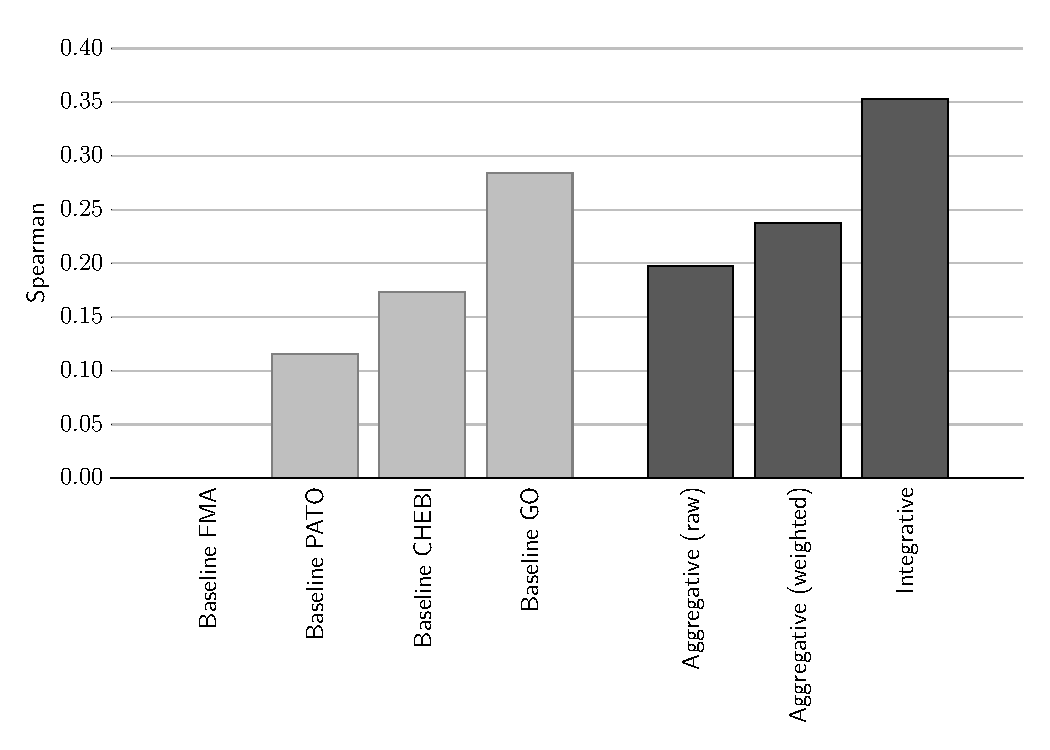
\includegraphics[width=0.9\linewidth]{images/biomodels-ferreira.pdf}
    \caption[Semantic similarity in the Biochemical Models dataset with~\boldmath$\ferreira$]{These results show the Spearman's rank coefficient between each semantic similarity measure and the gold-standard, measured with $\ferreira$ relatedness measure instead of $\sim[Resnik]$. In general, the multi-domain measures (shaded in a darker tone of grey) outperform the single-ontology ones (shaded in a lighter tone of grey).}
    \label{fig:biomodels-ferreira}
\end{figure}

One other aspect to consider in this case is the overall low correlation coefficient obtained with any of the measures and the multi-domain approaches. The best performance in all cases is obtained with $\ferreira$ with the \textbf{Integrative} approach, but this corresponds only to a correlation of~$0.352780$. Although not entirely statistically significant, I also calculated Pearson's correlation coefficient for these results, and obtained a value of~$0.581401$ for this case. A work by \citet{Hauke2011} shows that when Pearson's correlation coefficient is higher than Spearman's, then there is a (weak, at least) linear correlation between the two variables being measured (as opposed to other types of correlation): in this case, semantic similarity with the $\ferreira$ measure using the \textbf{Integrative} multi-domain approach, and the manual similarity values assigned by the Systems Biology expert. But a linear correlation with Pearson's coefficient of~$0.581401$ is still a low value. As such, the proposed measures seem to still be lacking in some way, as they do not properly reflect the expert assessment of similarity.

Fortunately, this result does not interfere with my hypothesis. The results presented in the figures of this section can still be used to show that multi-domain measures outperform single-ontology ones.

\begin{table}
\caption[Effect of cross-references on the performance of semantic similarity in the Biochemical Models dataset]{These results show the Spearman's rank coefficient between semantic similarity and the gold-standard, measured with $\ferreira$ relatedness measure. Each column reflects the results obtained without and with cross-references.}
\label{tab:epiwork-xref}
\centering
\small
\begin{tabular}{llcc}
\toprule
\multicolumn{2}{l}{\textbf{Measure}} & \textbf{No cross-references} & \textbf{With cross-references} \\
\midrule
Baseline    & \ontology{FMA}               & 0.000000 & 0.000000 \\
            & \ontology{PATO}              & 0.115841 & 0.115841 \\
            & \ontology{CHEBI}             & 0.173646 & 0.173358 \\
            & \ontology{GO}                & 0.283925 & 0.286247 \\
\addlinespace
\multicolumn{2}{l}{Aggregative (raw)}      & 0.197591 & 0.196394 \\
\multicolumn{2}{l}{Aggregative (weighted)} & 0.237164 & 0.239875 \\
\multicolumn{2}{l}{Integrative}            & 0.352780 & 0.359541 \\
\bottomrule
\end{tabular}
\end{table}
